\documentclass{article}
\usepackage{amsmath}
\usepackage{amsthm}
\usepackage{amssymb}
\usepackage{hyperref}
\usepackage[style=apa]{biblatex}
\usepackage[shortlabels]{enumitem}
\usepackage{graphicx}
\usepackage[margin=1in]{geometry}
\bibliography{sources.bib}
\usepackage{setspace}
\doublespacing

\DeclareMathOperator*{\argmax}{arg\,max}
\DeclareMathOperator*{\argmin}{arg\,min}

\newtheorem{theorem}{Theorem}[subsection]
\newtheorem{corollary}{Corollary}[subsection]
\newtheorem{lemma}{Lemma}[subsection]
\newtheorem{example}{Example}[subsection]
\theoremstyle{definition}
\newtheorem{definition}{Definition}[subsection]

\title{Investigating Hebbian Alternatives to Dense Associative Memory}
\author{Connor Hanley}
\date{\today}

\begin{document}
\maketitle

\begin{abstract}
  Dense Associative Memories generalize traditional Hopfield networks
  while providing a substantially increased capacity. This is achieved by increasing
  the separation of similarity scores between query patterns and stored patterns.
  The cost of increased capacity is simplicity and biological plausibility. We propose
  to investigate the capacity characteristics of a large subset of feasible Hebbian
  associative memories to see if there exists any alternative to
  Dense Associative Memories which maintains the simplicity and
  appeal of Hopfield networks.
\end{abstract}

\section{Introduction}

Humans are able to recognize and retrieve patterns of data using distorted,
noisy, and partial patterns \parencite{rumelhart_general_1986}. This
capacity of human memory is known as \textit{content-addressability}: patterns
which are stored in memory are able to be ``looked up'' by themselves or their
parts. Modeling this property is a classical task in computational cognitive
and neuroscience (see \textcites{marr_simple_1971,little_existence_1974,
amari_learning_1972,nakano_associatron-model_1972,stanley_simulation_1976}).
The family of models which implement content-addressability are known
as \textit{associative memory models} (AMs).
A recent revival of interest AMs in machine learning research,
driven by their equivalence with ``attention'' layers in the transformer
architecture \parencites{vaswani_attention_2023, ramsauer_hopfield_2021},
has led to drastic advances in the storage capacity of AMs
\parencites{demircigil_model_2017,krotov_dense_2016,hu_provably_2024}.

The foundational model for modern associative memory research is the
\textit{Hopfield network}
\parencites{hopfield_neural_1982,hopfield_neurons_1984}.
Hopfield networks are single-layer neural networks with full, lateral
connections.
This means that each artificial neuron in the network is connected with every
other neuron, except itself. Patterns that we wish to recall from the network
are stored in the connection weights between every other unit. Hopfield
networks learn new patterns to recall through a simple, biologically plausible
learning rule called the \textit{Activity Product Rule}
\parencite{haykin_neural_2009},
which is a kind of Hebbian update rule \parencite{hebb_organization_1949}.
The appeal of Hebbian update rules is that they are simple, in that they
are totally defined by local interactions between layers in neural networks
and they are biologically plausible, meaning that they have been observed in interactions
between biological neurons
\parencites{rolls_mechanisms_2013,bi_synaptic_1998,markram_regulation_1997}.

In spite of their simplicity and biological plausibility, Hopfield networks
are inherently flawed. The number of patterns that Hopfield networks
can store is pitifully small: with estimates in the range of $14\%$ to $15\%$
of the number of neurons in the network
\parencites{hopfield_neural_1982,amit_statistical_1987}.
In order to remedy the gap between the simplicity and plausibility of
Hopfield networks
and their child Dense Associative Memory models, we will theoretically derive
and empirically test the storage capacities of all Hebbian update rules
when used in single-layer neural networks with full lateral connections.

Discovering the limits of Hebbian alternatives to Dense Associative Memories
is not only desirable because of simplicity and biological plausibility
(while those are both laudable goals). For example, the study of
Vector-Symbolic Architectures, used for representing high-level cognitive-tasks
\parencites{smolensky_tensor_1990,plate_holographic_1995,gayler_multiplicative_1998},
requires an auto-associative memory ``clean-up memory''. This means that
the expressive capabilities of Vector-Symbolic Architectures are
affected by the capacity of the associative memory used.

In the following we will discuss the problem in more depth. To do
this, we will first
lay out the theoretical motivation: beginning with an introduction to
the literature
in \autoref{sec:background}, covering associative memories in
\autoref{sec:associative-memories},
Hopfield networks in \autoref{sec:hopfield-networks}, their generalization with
Dense Associative Memories in \autoref{sec:dense-associative-memory},
and Hebbian learning rules in \autoref{sec:hebbian-learning-rules}. We will restate the
problem of Hebbian Dense Associative Memories in \autoref{sec:hebbian-dam}, and
provide a work plan in \autoref{sec:work-plan}. Finally, we will discuss
the timeline for completing this project in \autoref{sec:timeline}.

\section{Background}\label{sec:background}

In order to understand the need for a Hebbian alternative to Dense Associative
Memories, we must first familiarize ourselves with the literature up to this
point. Associative Memory research has a wealth of literature and alternatives.
In order to limit the scope of this research, we limit ourselves only to the
family of models based on Hopfield networks \parencite{hopfield_neural_1982}.

\subsection{Associative Memories}\label{sec:associative-memories}

An associative memory, in particular an \textit{auto}-associative memory,
is a general structure that can be implemented by many mathematical
and computational objects. Broadly speaking, an associative memory is a
tuple of a set of objects $\mathcal X$, called the set of
\textit{traces} or \textit{stored patterns},
and a (typically learned) identity map over the set of stored
patterns, $T: \mathcal X \to \mathcal X$.
More formally,

\begin{definition}
  An (auto) \textit{associative memory} is a tuple $\langle \mathcal
  X, T \rangle$, where
  \begin{enumerate}[(a)]
    \item $\mathcal X$ is a set of objects, called the
      \textit{pattern} set, or set of \textit{traces}, typically
      high-dimensional vectors; and,
    \item The \textit{recall function}, $T$, maps from the set
      of traces back to
      the set of traces, such that $T(x) \approx x$, for all $x \in
      \mathcal{X}$,
      and $T(\overline x) \approx x$, where $\overline x$ is a
      perturbed, masked, or degraded form of $x \in \mathcal{X}$.
  \end{enumerate}
\end{definition}

We will be assuming throughout that the pattern set is the set of rows
of the \textit{pattern matrix} $\Xi = [\xi^1, \xi^2, \dots, \xi^N]$,
where each \textit{stored pattern} $\xi^i \in \{-1, 1\}^D$. It is sufficient
to specify the pattern matrix, or the sequence of patterns, for an
associative memory,
and it should be assumed that the pattern set is just composed of the
rows of the pattern matrix.
Associative memories are \textit{content-addressable}, as their recall function
is able to recover desired associated patterns from partial information
\parencites{mcclelland_appeal_1986,haykin_neural_2009}. This is in
contrast to memory models which recall information based on arbitrary
associations, like indices into memory locations.

While it is not essential to the most general definition of
associative memories,
we usually desire that the recall function be learned. Furthermore,
associative memories have a maximum capacity of traces that they can store.

\begin{definition}[Retrievability; Capacity]
  Following \textcite{bao_capacity_2022}, let us have an associative
  memory with patterns
  $\xi^1, \xi^2, \dots, \xi^N$, where each element $\xi^i_j$ is
  $-1$ or $1$ with equal likelihood. For any $\delta < 0.5$, we define
  the $\delta$-perturbation of $\xi^i$, denoted by $\bar \xi^i$, as
  the $D$-dimensional vector $\xi^i$ with each element flipped with a likelihood
  of $\delta$. Then, we say that the set $\xi^1, \xi^2, \dots, \xi^N$ is
  $(\delta, \varepsilon)$-retrievable if for every $\xi^i$, $i = 1, 2, \dots, N$
  it is such that:
  \begin{equation}
    \mathbb{P}(T(\bar \xi^i) \neq \xi^i) < \varepsilon.
  \end{equation}
  The \textit{capacity} $C$ of the associative memory is the maximum
  cardinality of the pattern set such that all patterns are $(\delta,
  \epsilon)$-retrievable.
\end{definition}

In \textcite{krotov_dense_2016}, capacity is denoted by $N^{\max}$, where
$N$ is the first dimension of the pattern matrix. Associative memory
capacity is affected by the (1) kind of data being stored,
i.e. if the data
has a high pairwise correlation, which leads to ``cross-talk''
\parencite{kohonen_correlation_1988},
(2) the dimensionality of the data, and (3) the implementation of the
recall function $T$.
For example, if the associative memory is a neural network with
tensor weights \parencite{kelly_memory_2017},
then the capacity scales with the number of the weights
\parencite{little_analytic_1978} (expanded
further in \autoref{sec:dense-associative-memory}).

Before Hopfield networks, there were Correlation Matrix associative memories.
So-called, because they relied on dot-product correlations for recall.
\begin{example}[Correlation Matrix associative
  memory]\label{example:correlation}
  Let us have a pattern matrix $\Xi = [\xi^1, \xi^2, \dots, \xi^N]$ of
  vectors sampled from $\{1, -1\}^D$. The Correlation Matrix associative memory
  recall function is of the form:
  \begin{align}
    T(x) &= g \left(\sum^N_{\mu=1} \xi^\mu \left( \sum^D_{i=1}
    \xi^\mu_i x_i \right)\right) \nonumber \\
    &= g \left( \Xi^\top \Xi x  \right),
  \end{align}
  where $g$ is an ``activation function'', typically \textit{signum} %% need to define signum
  for binary vectors.
\end{example}

\begin{example}\label{example:argmax-am}
  Like above, let us have a pattern matrix $\Xi = [\xi^1, \xi^2,
  \dots, \xi^N]$ of
  vectors sampled from $\{1, -1\}^D$. Let our recall function $T$ be:
  \begin{equation}
    T(x) = \xi^i,~\text{where}~i = \argmax_{i \in [1, N]}
    [\text{sim}(\xi^i, x)],
  \end{equation}
  where $\text{sim}$ is some similarity function \parencite{kelly_memory_2017},
  e.g. the cosine similarity or Hamming distance.
\end{example}

\begin{example}[Minerva2]\label{example:minerva2}
  Minerva2 \parencite{hintzman_minerva_1984} is an associative memory
  used in cognitive
  science which is about as old as Hopfield networks. As per usual, we have
  binary patterns $\Xi = [\xi^1, \xi^2, \dots, \xi^N]$. The recall function is:
  \begin{equation}
    T(x) = \text{sgn} \left[ \sum^N_{\mu=1} \xi^\mu \left(
    \frac{\sum^D_{i=1} \xi^\mu_i x_i}{\|\xi^\mu\| \|x\|} \right)^3 \right].
  \end{equation}
\end{example}

\subsection{Hopfield Networks}\label{sec:hopfield-networks}

Hopfield networks
\parencites{hopfield_neural_1982,hopfield_neurons_1984} are an associative
memory with deep connections to Example \ref{example:correlation},
except that they
understand their recall function in terms of an \textit{energy} function:

\begin{definition}\label{def:hopfield-nets}
  \textit{Hopfield networks} are single-layer neural networks of $D$ computational units
  with full, lateral connections. The state of the network is described
  by the state vector $\sigma$ at time $t$, denoted by $\sigma^{(t)}$.
  The \textit{energy} of the network, $E (\sigma^{(t)})$ is:
  \begin{equation}
    E(\sigma^{(t)}) = - \frac{1}{2} \sum^N_{\mu=1} \left(\sum^D_{i=1}
    \xi^\mu_i \sigma^{(t)}_i\right)^2.
  \end{equation}
  Let $\sigma[i := b]$ be the vector $\sigma$, with the $i$'th
  component set to $b$. Then,
  update rule for the state of the network is:
  \begin{equation}
    \sigma^{(t+1)}_i = \text{sgn} \left[ E(\sigma^{(t)}[i : = -1]) -
    E(\sigma^{(t)}[i := 1]) \right].
  \end{equation}
\end{definition}

After setting the initial state at time $t=0$, the network
continuously updates random
elements of the state vector depending upon whether the update lowers
the energy of the
network. The energy function, then, forms a ``landscape'', where
local minima in the space
(ideally) correspond with desired patterns to be stored (see \autoref{fig:energy-landscape}).

\begin{figure}
    \centering
    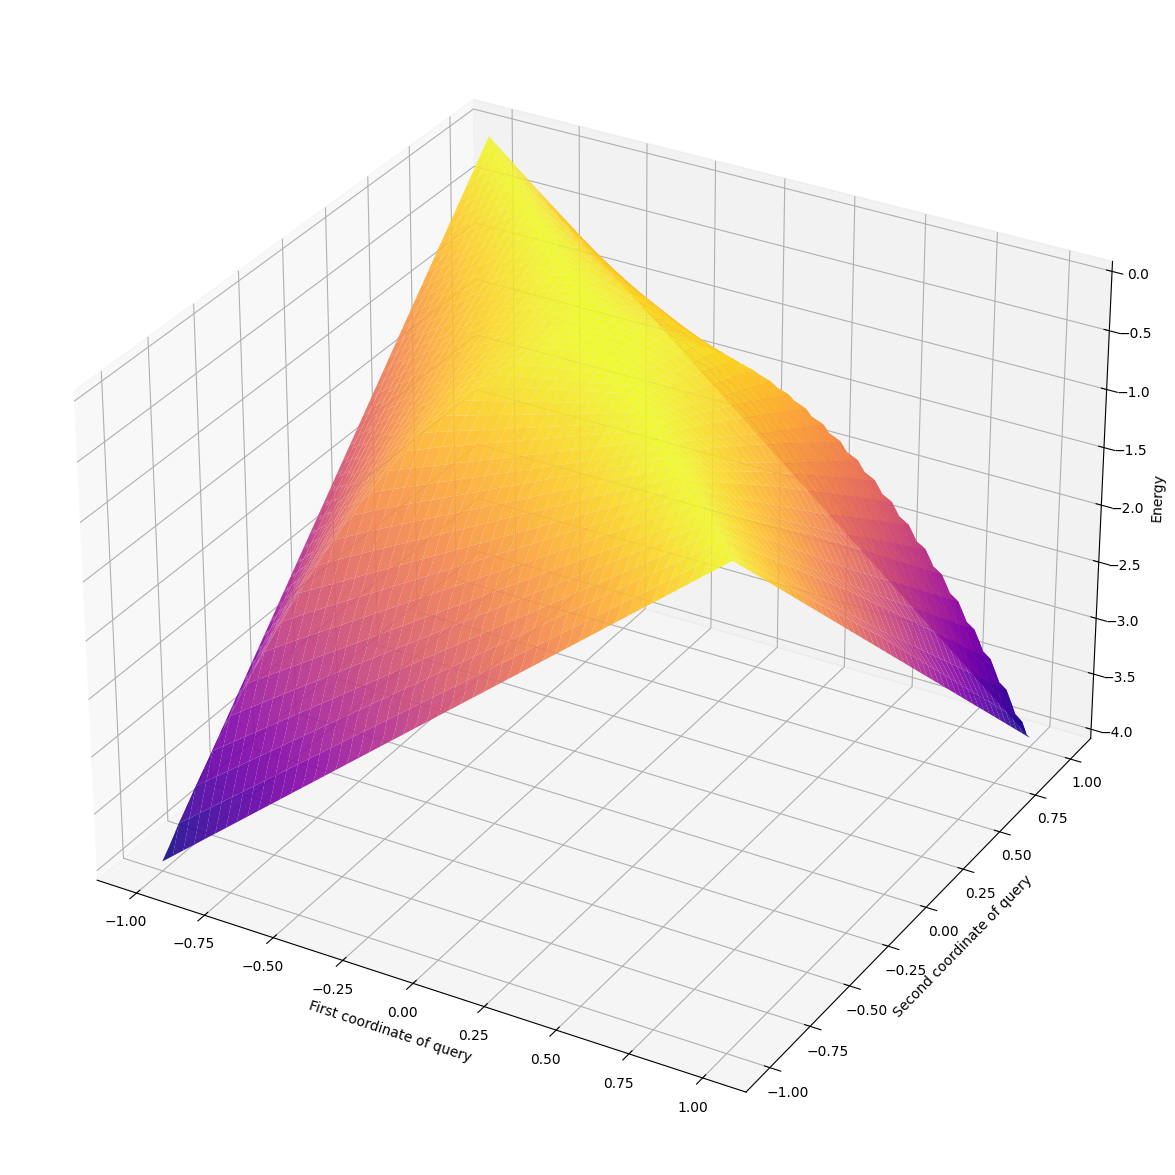
\includegraphics[width=0.5\linewidth]{energy_landscape.png}
    \caption{Energy landscape of Hopfield network storing $[-1,-1]$ and $[1,1]$.}
    \label{fig:energy-landscape}
\end{figure}

While the use of the energy function seems at odds with our definition
of associative memories, we can align the two by considering a
single-pass variant of the energy-minimization. It can be shown
that updating every element $i$ of the state vector $\sigma^{(t)}$
in a single pass (synchronously) corresponds with the update rule
\parencite{krotov_modern_2025}:
\begin{equation}\label{eq:hopfield-sync}
  T(\sigma) = \text{sgn} \left[ \sum^N_\mu \xi^\mu \left(
  \sum^D_{i=1} \xi^\mu_i \sigma_i \right) \right],
\end{equation}
which is just the update rule of Correlation Matrix associative memories
(see, Example \ref{example:correlation}).

%% NOTE: need to improve the discussion here:
%% 1. linking to the next section
%% 2. what's so cool about hopfield networks? what inspired continued
% work on them?
%% 3. what are some applications of hopfield networks across the
% sciences, make sure
%%    to name drop some cognitive applications
Hopfield networks unfortunately have a pitifully low
storage capacity: the critical capacity $C$ being around $14\%$ to $15\%$
of the number of neurons in the model
\parencites{amit_statistical_1987,hopfield_neural_1982}. As a computational
model of human memory this will not do.  %% why?
Likewise, this is unsuitable for machine learning tasks involving large
datasets, e.g. large language models. Capacity problems led researchers
to investigate how one can improve the capacity of Hopfield networks,
while maintaining the simplicity and interpretability of energy minimization.

\subsection{Dense Associative Memories}\label{sec:dense-associative-memory}

Dense Associative Memory models are a generalization of Hopfield networks that
maintain energy minimization in recall, but have a dramatically
increased storage capacity \parencite{krotov_dense_2016,demircigil_model_2017}.
Instead of relying on full lateral connections between units in a
single dimension,
Dense Associative Memories either have multiple connections between
computational units, or, increase the number of layers present in the model.
\textcite{krotov_large_2021} notes that this is to be expected, given the
information limits of single neurons.

\begin{definition}
  Given binary patterns $\xi^1, \xi^2$, $\dots, \xi^N$ sampled from
  $\{-1, 1\}^D$,
  a \textit{Dense Associative Memory} is characterized by:
  \begin{enumerate}[(i)]
    \item A $D$-dimensional \textit{state vector} at time $t$, denoted by $\sigma^{(t)}$;
    \item A \textit{polynomial transmission function} $F_n$, where:
      \begin{equation}
        F_n (x) = \frac{1}{n} (x)^n;
      \end{equation}
    \item An \textit{energy function} of the state of the network at time $t$,
      \begin{equation}
        E(\sigma^{(t)}) = \sum^N_{\mu=1} F \left( \sum^D_{i=1}
        \xi^\mu_i \sigma^{(t)}_i \right);
      \end{equation}
    \item An update equation for the state of the network, such that:
      \begin{equation}
        \sigma^{(t+1)}_i = \text{sgn} \left[ E(\sigma^{(t)}[i := -1])
        - E(\sigma^{(t)}[i := 1]) \right].
      \end{equation}
  \end{enumerate}
\end{definition}

Like Hopfield networks, the state vector update rule is typically
performed asynchronously.
However, we can define a synchronous update rule which makes the
Dense Associative
Memory an Associative Memory with update rule:
\begin{equation}
  T(\sigma) = \text{sgn} \left[\sum^N_{\mu=1} \xi^\mu F_n' \left(
  \sum^D_{i=1} \xi^\mu_i \sigma_i \right)\right],
\end{equation}
where $F_n'$ is the derivative of $F_n$. From this definition we immediately
see how this framework generalizes Hopfield networks.

\begin{example}
  Hopfield networks in Definition \ref{def:hopfield-nets} are Dense
  Associative Memories
  with polynomial transmission function $F_2$.
\end{example}

\begin{example}
  Minerva2 (from Example \ref{example:minerva2}) are roughly Dense
  Associative Networks,
  assuming that all patterns $\xi^1, \xi^2, \dots, \xi^N$ and query
  patterns are normalized,
  and with polynomial transmission function $F_4$.
\end{example}

Dense Associative Memories improve the storage capacity of Hopfield networks
in that the capacity $C$ of a Dense Associative Memory, with
polynomial function $F_n$,
and dimensionality of patterns $D$ is:
\begin{equation}
  C \propto D^{n-1}
\end{equation}
\parencites{krotov_dense_2016,demircigil_model_2017,bao_capacity_2022}.
The increased capacity comes from the ``steeper'' energy basins
around minima corresponding to patterns stored in the network, which
is brought about by the exponentiation of the dot product similarity
between the stored patterns and the query pattern (for discussion, see
\textcite{kelly_memory_2017}). Memory capacity for Dense Associative
Memories can also be increased by making more domain sensitive
similarity functions \parencite{millidge_universal_2022},
e.g. with kernel estimation \parencite{hu_provably_2024,wu_uniform_2024}.

\begin{figure}
    \centering
    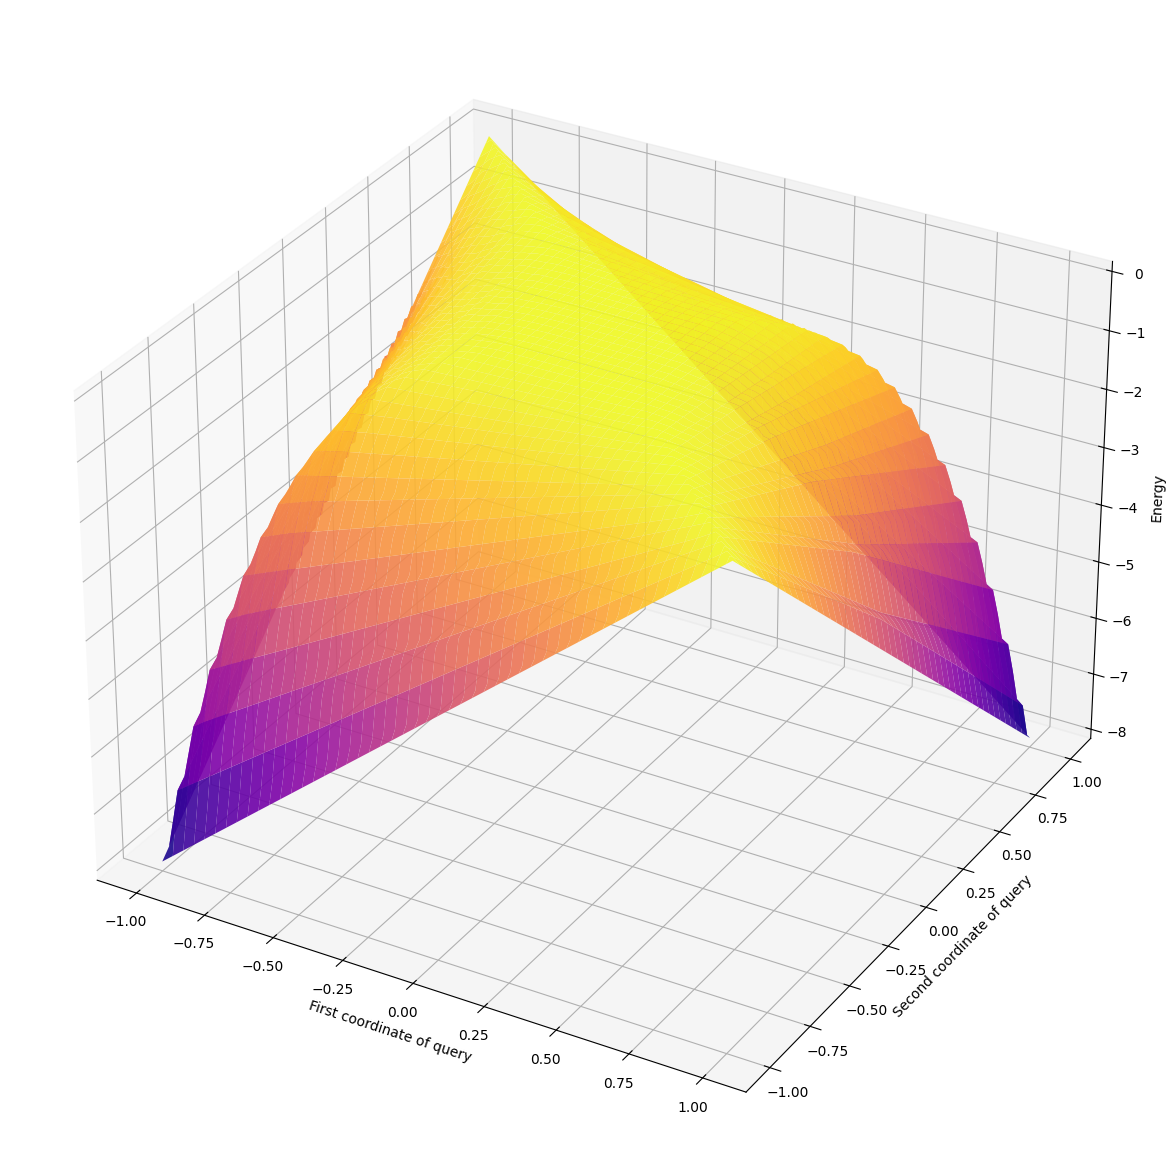
\includegraphics[width=0.5\linewidth]{energy_landscape_minerva.png}
    \caption{Energy landscape of Dense Associative Memory with $F_4$.}
    \label{fig:energy-landscape-minerva}
\end{figure}

In spite of the enormous gains in capacity using non-linear
transmission functions, Dense Associative Memories lose the ability
to be interpreted as simple one-layer networks with lateral connections
and trained via Hebbian update rules
\parencites{krotov_large_2021,mcalister_sequential_2025}.
On the one hand, this is to their benefit: a continuous variant of
Dense Associative
Memory called \textit{Modern Hopfield Networks} has been shown to be
equivalent to multi-head attention in Transformer neural networks
\parencites{ramsauer_hopfield_2021,vaswani_attention_2023}. Likewise,
the framework behind Dense Associative Memories has been developed for
modular neural network architectures \parencite{krotov_hierarchical_2021},
and has been used to define an \textit{Energy Based Transformer}
\parencite{hoover_energy_2023}, as well as contribute to the interpretability
of Diffusion Models \parencite{pham_memorization_2025}.

%% EXPAND HERE
But the cost is their simplicity and biological plausibility.
Correlation matrix memories
trained with Hebbian update rules mimic observed phenomena in
biological neural networks; meaning that they perform computations
which are in principle achievable by biological systems.

\subsection{Hebbian Learning Rules}\label{sec:hebbian-learning-rules}


Hebbian learning rules are a family of weight update rules for both
artificial and spiking neural networks which posit that
the weights connecting two local layers are determined entirely
by the activity of just those two layers
\parencites{hebb_organization_1949,sejnowski_hebb_1989}.
We can define Hebbian learning rules in the most general sense:
\begin{definition}[Hebbian learning rule]\label{def:hebbian-learning-rule}
  Consider a neural network with layers with $N$ layers $x_{1}, x_2,
  \dots, x_N$,
  and for each layer and the layer above ($i$ and $i + 1$, $i \neq N)$, there
  is a \textit{weight matrix} $W_{ij}$. Then, a Hebbian learning rule for this
  network is an update rule for layers $i, j$, where $j = i + 1$, such that:
  \begin{equation}
    \Delta W^{ij} = F(W^{ij}; x^i, x^j).
  \end{equation}
\end{definition}

Hebbian learning rules are \textit{entirely local}, as we can see from
the requirement that the learning rule only affect layers $i$ and $j = i + 1$.
In their simplest formulation, Hebbian learning rules are not
all error-correcting \parencite{munakata_how_2006},
which is in contrast to popular learning algorithms
like back-propagation of error \parencite{rumelhart_learning_1986}. However,
there is a local learning paradigm, called Predictive Coding (for review see
\textcite{spratling_review_2017}), which
has implemented associative memories in deep neural networks
\parencite{salvatori_associative_2021}

The simplest method for training Hopfield networks (and Correlation
  Matrix associative
memories) is to use the Activity Product Rule \parencite{haykin_neural_2009}.

\begin{definition}\label{def:activity-product}
  The \textit{Activity Product Rule} is a Hebbian learning rule defined
  for layers $x^i$ and $x^j$, $j = i+1$, with weights $W^{ij}$, such that:
  \begin{equation}
    \Delta W^{ij} = \eta x^i (x^j)^\top,
  \end{equation}
  where we call $\eta$ the \textit{learning rate}.
\end{definition}
\noindent
To train Hopfield networks using the Activity Product Rule,
let us have patterns $\xi^1, \xi^2, \dots, \xi^N$; a single
$D$-dimensional layer $\sigma$, and full lateral weights between $\sigma$
and itself called $W$. At training step $t=0$, we initialize $W$
to be all zeros:
\begin{equation}
  W^{(t=0)}_{ij} = 0.
\end{equation}
Then, for each new time step from $t=1$ to $t = N$, we produce a new
pattern to the weights for it to memorize, updating it with
the Activity Product Rule:
\begin{equation}
  W^{(t+1)} \gets W^{(t)} + \eta \xi^{t+1} (\xi^{t+1})^\top.
\end{equation}Hopfield networks learn with the Activity Product Rule
\parencite{haykin_neural_2009}.
Talk about biological evidence for Hebbian learning rules. Stress simplicity.
If $\eta = 1$, then we get a weight matrix $W$ which is a
linear combination of all the desired patterns we wish to store:
\begin{equation}
  W^{(t=N)} = \sum^N_{\mu=1} \xi^\mu (\xi^\mu)^\top.
\end{equation}
Weights trained in this way makes the synchronous recall function $T$
for the Hopfield network a linear combination of the stored patterns
weighted by their dot product similarity with the query pattern:
\begin{equation}
  T(\sigma) = \text{sgn}\left[W^{(t=N)} \sigma \right] =
  \text{sgn}\left[ \sum^N_{\mu=1} \xi^\mu (\xi^\mu)^\top \sigma\right].
\end{equation}

In principle, auto-associative memories could be trained with
\textit{other} Hebbian update rules, as long as the Hebbian update
rule was additive and can be understood as reducing the energy of the network
(according to some rule). More strictly, a learning rule is additive when,
after training, the weights are of the form:
\begin{equation}
  W^{(t_\text{final})} = \sum^N_{\mu = 1} f(W; \xi^\mu (\xi^\mu)^\top).
\end{equation}
This property is required in order to maintain the neural interpretation
of recall, as post-multiplication distributes over element-wise addition.
The second important property of the weight update rule is that it reduces
some natural energy function for the update rule. For example, if we derive the
energy rule through the relation from \textcite{krotov_hierarchical_2021}.

Given that $f$ in
Definition \ref{def:hebbian-learning-rule} is a large class of functions,
we will restrain ourselves to only functions of the following form:
\begin{definition}\label{def:expanded-learning}
  The \textit{expanded} Hebbian learning rule is the Taylor expansion
  of the weight update rule about $(0, 0)$
  \parencite{gerstner_mathematical_2002}:
  \begin{align*}
    \Delta W_{ij} &= f(W_{ij}; x_i, x_j) \\
    &= f(W_{ij}; 0, 0) + \frac{\partial f}{\partial x_i} \big|_{(0,
    0)} x_i + \frac{\partial f}{\partial x_j}
    \big|_{(0, 0)} x_j \\
    &+ \frac{1}{2} \frac{\partial^2 f}{\partial v^2_i} \big|_{(0, 0)}
    x_i^2 + \frac{1}{2} \frac{\partial^2 f}{\partial v^2_j}\big|_{(0,
    0)} x_j^2 \\
    &+ \frac{\partial^2 f}{\partial x_i \partial x_j}\big|_{(0, 0)}
    x_i x_j + \mathcal{O}(x).
  \end{align*}
  We denote the Taylor coefficients by
  $c_n^{\{\text{corr},~\text{pre},~\text{post}\}}$, with
  $n$ denoting the order of the coefficient, $\text{corr}$ denoting
  the coefficient
  weighting the correlation between the pre- and post-synaptic neural
  layers, and
  $\text{pre}$ and $\text{post}$ to denote the coefficients of the
  pre- and post-synaptic
  layers themselves (respectively).
  This gets us:
  \begin{align*}
    \Delta W_{ij} &= f(W_{ij}; x_i, x_j) =
    c_0 (W_{ij}) + c_1^\text{pre} (W_{ij}) x_j + c_1^\text{post} x_i \\
    &+ c_2^\text{pre} (W_{ij}) x_j^2 + c_2^\text{post} (W_{ij}) x_i^2
    + c_2^\text{corr} (W_{ij}) x_i x_j \\
    &+ \mathcal{O} (x).
  \end{align*}
\end{definition}

This definition immediately gives us the following:
\begin{example}
  The Activity Product Rule (Definition \ref{def:activity-product}) is
  just the expanded Hebbian learning rule with $c_2^\text{corr}$
  set to some constant, and all other constants set to $0$.
\end{example}

\begin{example}
  \textit{Oja's Rule} \parencite{oja_simplified_1982}
  by setting $c_2^\text{corr} = \eta_0 > 0$,
  and $c_2^\text{post} = - \eta_0 w_{ij}$, with all other
  coefficients set to $0$.
\end{example}

\section{Hebbian Dense Associative Memory}\label{sec:hebbian-dam}

Instead of manipulating the similarity kernel to increase
memory capacity (as in \textcite{hoover_dense_2024,hu_provably_2024}),
can we use different Hebbian learning rules for
single-layer associative memories to
achieve similar capacities to Dense Associative Memories? Preliminary
investigation into a subset of Hebbian learning rules
found that the capacity characteristics broadly followed the
derived capacity of traditional Hopfield networks
\parencite{lansner_benchmarking_2025}. But does this result
hold true for all Hebbian learning rules?

\subsection{Work Plan}\label{sec:work-plan}

Determining the capacity characteristics of Hebbian networks
involves two components. The first is to provide theoretical reasoning
as to the capacity of associative memories. The second is to
provide experimental evidence of the theoretical reasoning on
large-scale associative memory tasks: namely, pattern reconstruction
and utility in a larger network.

\subsubsection{Theoretical Work}

We have seen above that we have proofs of the capacity of
Hopfield networks and Dense Associative Memory. A contemporary
example of this kind of proof can be found in \parencite{bao_capacity_2022},
which proves capacity with respect to a perturbation of a query
and a lower probability bound of error in recall.

Proving the capacity characteristics of Hebbian networks ought to
follow the same formula. Given that the class of Hebbian update rules
is large, we will focus in on a few learning rules: namely,
the learning rules which were experimentally tested in
\textcite{lansner_benchmarking_2025}, and then the expanded
form in Definition \ref{def:expanded-learning}. The goal of this
part of the project is to come up with a theorem that shows that,
with coefficients $c_1, c_2, \dots, c_n$, that the Hebbian
auto-associative memory has a capacity $C$ which is some
function of the dimensionality of the patterns stored
(see Equations (1-6) in \textcite{lansner_benchmarking_2025}, or
Theorem 1 from \textcite{bao_capacity_2022}).

The proof strategy is the following: suppose
that we have a learning rule with coefficients $c_1, c_2, \dots, c_n$,
denoted by $\mathcal{L}_{c_1, c_2, \dots, c_n}$. Further, suppose
that we have patterns $\xi^1, \xi^2, \dots, \xi^N$, where
each element of $\xi^\mu$ is either $-1$ or $1$ with equal probability.
Let $T(x)$ be the recall function of an associative memory with learning
rule $\mathcal{L}_{c_1, c_2, \dots, c_n}$. We define capacity in
the same way as \textcite{bao_capacity_2022}, i.e., in relation
to a perturbation constant $\delta < 0.5$ and an error threshold $\varepsilon$.
We must prove the maximum $N$ (number of patterns) which are
all one-step $(\delta, \varepsilon)$-recoverable. This means that
$N$ is the maximum number of patterns such that, for every pattern stored,
the probability of a one-step recall of perturbation of the pattern
not being equivalent to the pattern itself is less than $\varepsilon$:
\begin{equation}
  \mathbb{P}(T(\bar \xi^i) \neq \xi^i) < \varepsilon, ~\forall i \in [1, N],
\end{equation}
with $\bar \xi^i$ denoting the $\delta$-perturbation of $\xi^i$.

Having a proof of this form is desirable as it allows to fairly compare
Hebbian associative memories with other kinds of associative memories.
Merely providing estimated scaling characteristics for
the capacity of networks, as in \textcite{lansner_benchmarking_2025}, does
not account for potential problematic elements in the kinds of patterns
being memorized. For example, MNIST \parencite{lecun_mnist_2010}
images, naively represented, are all highly correlated with one another.
This ``cross-talk'' \parencite{kohonen_correlation_1988} can lead
to spurious similarity measures between query patterns and estimated
patterns.

\subsubsection{Experimental Work}

Purely theoretical work is well and good. But the proof of the
pudding is in the eating,
and it is important to test the derived results for their accuracy to
the real world.
In order to verify our estimates, the goal will be to subject generated Hebbian
associative memories to large-scale tasks. The most intuitive and popular
task for associative memories is pattern reconstruction. Likewise, in order
to see how these networks fair in real-world scenarios, integrating
derived models in a larger architecture for the same task will provide
an equal playing field for comparison.

Pattern reconstruction tasks are often included in the demonstration of
associative memory capacities. Oftentimes, however, the demonstrations
are merely qualitative. If the model can produce estimated patterns that
look sufficiently similar to our eyes to the original query, then they succeed.
But this is hardly objective, and so we require a better measure of
reconstruction.
In order to have an objective pattern reconstruction test, we need to
have a shared basis in order to compare results. This is some
distance metric for patterns, a function which gives us the similarity
between a presented pattern and its output from the network. One common
measure of similarity in Vector-Symbolic Architectures 
\parencites{smolensky_tensor_1990,plate_holographic_1995,gayler_multiplicative_1998}
is \textit{cosine similarity}:
\begin{equation}
  \text{sim}(x, y) = \frac{x \cdot y}{\|x \| \|y \|},
\end{equation}
which is the normalized dot-product between two vectors. This gives us the 
angle in $D$-dimensional space between the two vectors, where $\text{sim}(x, y) = 1$
means that the vectors are \textit{orthogonal}. Preliminary experimentation
with traditional Hopfield networks showed that, at or above critical capacity
with the MNIST dataset, Hopfield models produce spurious states which have
a high cosine similarity to all memorized patterns.
To overcome this, it seems prudent to test similarity using a battery of 
similarity measures: for review, we can use those listed in 
\textcite{kelly_memory_2017}. 

%% I think it would be cool to insert the associative memory in 
%% one of the models that u use minerva2 in? What are your thoughts

\section{Timeline}\label{sec:timeline}

%% Going to create a Gantt chart here, I think? Still under work
Theoretical work should be done by Christmas. Experimental work likewise
requires only a couple of months. Data science certification requires emphasis
here on large-scale projects. So, I would like to rigorously examine
each model on a variety of tasks. One to two papers arises from this project:
one talking about the theory of Hebbian DAM, and the other part including
the experimental work. It would be better for a single paper, but if that
runs too long, then experimental work can be a part 2.

\printbibliography
\end{document}
